\documentclass[hidelinks,11pt]{article}
\usepackage{graphicx}
\usepackage{hyperref}
\usepackage{xcolor}
\usepackage{amsmath}
\usepackage{glossaries}
% \makeglossaries

% \newglossaryentry{latex}
% {
%     name=latex,
%     description={Is a mark up language specially suited 
%     for scientific documents}
% }

% \newglossaryentry{maths}
% {
%     name=mathematics,
%     description={Mathematics is what mathematicians do}
% }

\title{Quantum Machine Learning}
\author{Hamza, Ali; Hoda, Bilal}
\date{\today}



\begin{document}
\maketitle
\begin{center}
		
	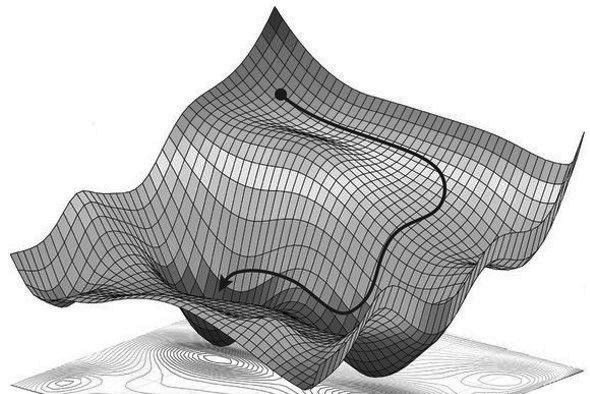
\includegraphics[scale = 0.7]{images/title2.jpg}

\end{center}

\newpage

\tableofcontents
\newpage

\section{Abstract}

*This section has been left to be completed at the end of the report
\newpage
\section{Introduction}

The data that we observe can be generally explained by an underlying process.
However, the vast amount of data that we observe around us leaves us benign of any patterns that may emerge from that data. For instance, we can observe that consumer behaviors are cyclical and their purchase histories follow a certain trend. To expound, we can see that people do no buy warm clothes all year round, or consume the same food all year round. While these trends are easy to observe, humans tend to miss many trends that machines can easily detect. 
\paragraph{}
Machines are extremely good at crunching data, thus using data to approximate a certain trend within it makes obseving those trends much easier. While approximations may not preesent us the complete picture due to the many irregularities present within the data, we are still able to infer a certain trend from it. This is where machine learning comes in. These trends or patterns may help us understand the correlations within the data and by consequence help us infer a causation for that trend. This allows us to then predict human behavior, and other trends in data based on the assumption that these trends are consistent and are not subject to a lot of change \cite{BOOK:3}.
\subsection{What is Machine Learning?}

	\textit{Machine Learning (ML)} is the field of study that involves techniques that allow machines to learn from large samples of data. Machine Learning is a broad term that encompasses a wide variety of techniques to characterize and classify data that then aids us in making decisions by predicting outcomes of new data. Generally Machine Learning involves training a machine using a learning algorithm that takes data set as input outputs a certain classification, ir characterisitic of the data. Machine learning solutions are currently widespread in the classical paradigm of computing, and generally rely on classical data sets.\cite {inproceedings}
	\paragraph{}
	\paragraph{}
	\subsubsection{Learning Methodologies}
	In terms of learning mathodologies, machine learning is generally divided into three categories: 
	\begin{itemize}
		\item \textbf{Supervised Learning}\paragraph{}
		This method involves the use of a data set that is comprised of input and corresponding output vectors. A very common dataset of this category is used in training machines to recognize handwritten digits. Once the machine goes through enoug data, it becomes aware of trends within the handwritten data and is then capable of recognizing new handwritten data and map it to the right digit. \cite{BOOK:3} 
		\item \textbf{Unupervised Learning}\paragraph{}
		This method involves the use of unstructured training data that consists of a set of input vectors $x$ without any corresponding target values. The goal may be to discover groups of similar examples within the data, where it is called \textit{clustering}, or to determine the distribution of data within the input space, known as \textit{density estimation}, or to project the data from a high-dimensional space down to two or three dimensions for the purpose of visualization.\cite{BOOK:3} 

		\item \textbf{Reinforcement Learning}\paragraph{}
		This method involes the use of a reward system that trains the machine to better optimize itself for better predictions. The machine is given input vectors that it must utilize to discover patterns and trends within the data via trial and error. There is a sequence of states and actions in which the learning algorithm is interacting with its environment. In many cases, the current action not only affects the immediate reward but also has an impact on the reward at all subsequent time steps. For instance, by using appropriate reinforcement learning techniques a \textit{neural network} can learn to play the game of backgammon to a high standard. Here the network must learn to take a board position as input, along with the result of a dice throw, and produce a strong move as the output. This is done by having the network play against a copy of itself for a large number of games.\cite{BOOK:3} 
	\end{itemize}
	

\subsection{What is Quantum Machine Learning?}

*This section has been left to be completed at the end of the report

\newpage
\section{Classical Machine Learning Algorithms}
\subsection{Gradient Descent}

	Machine Learning often relies on optimization to obtain results that are to make use of complex classification problems, such as curve fitting, pattern recognition, etc. These are built upon a cost/loss function that makes use of the present data. The purpose of a cost function is to optimize the present function so that it presents us with the most accurate classification of the data. \textit{Gradient Descent}.
	\paragraph{}
	Gradient Descent uses approximation and calculus to find the global extremes of a function, $f(x)$, where $x$ is an N-Dimensional vector. The purpose of using gradient descent instead of differentiation is simple. Not all curves are well defined functions and thus through a simple recursive algorithm, finding the extreme values of the curve become relatively easy. 
	\paragraph{}
	Let us begin by making use of analogy. Suppose you're at the top of the mountain and want to get to the bottom in the least amount of steps. Since you're in a 3D space, you can only move in the x, y or some combination of the two vectors. Through, Gradient Descent you can find the best step which has the highest rate of decrease in altitude. This process is then repeated until the decrease caused by the steepest step is approaches a very small value $\approx 0$ Random citation \cite{BOOK:1} 
	\paragraph{}
	[12] The mathematical definition of this algorithm is as follows:  
	$$f(x_i, y_i) = f(x_{i-1}, y_{i-1} - \alpha\nabla f(x_{i-1}, y_{i-1})$$


\subsection{Support Vector Machines}
	Machine Learning algorithms are also good at classification problems. This involves looking at a data set and identifying \textit{clusters} or similar characterisitics within the data to group and classify it.
	\paragraph{}
	Support Vector Machines (SVM) is a supervised machine learning algorithm used for linear discrimination problems. Our goal is to find an optimal \textit{hyperplane} which maximizes the margin such that it discriminates between classes of feature vectors and is used as a decision boundary for future data classification. The SVM is formulated as maximizingthe distance between the hyperplane and closest data points called support vectors. The objective function could be convex or non-convex depending on the kernel used in SVM algorithm.\cite {BOOK:1}

	\begin{center}
	    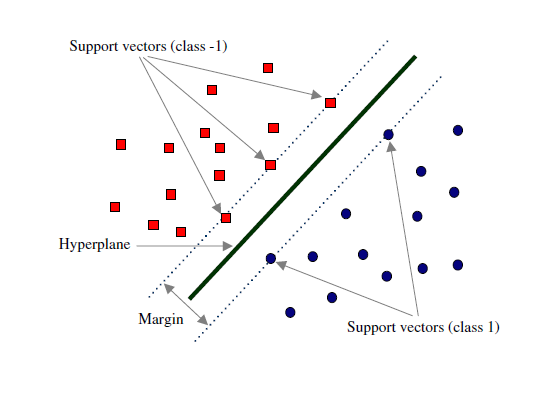
\includegraphics[scale = 0.7]{images/hyperplane.png}
	    Figure: Hyperplane [4]
	\end{center}

	We have l training examples where each example x are of D dimension and each have labels of either y=+1 or y= -1 class, and our examples are linearly separable. Then, our training data is of the form,
	\begin{center}
	    $\{x_i,y_i\}$ where i = 1 ... L, $y_i \in \{-1,1\}$, x $\in$ $R^D$ 
	\end{center}

	If the number of input features is 2, then the hyperplane is just a line. If the number of input features is 3, then the hyperplane becomes a two-dimensional plane. It becomes difficult to visualize when the number of features exceeds 3.
	Support vectors are data points that are closer to the hyperplane and influence the position and orientation of the hyperplane. Using these support vectors, we maximize the margin of the classifier. Deleting the support vectors will change the position of the hyperplane.[5]
	\\

	We define a linear discriminate function as;
	\begin{center}
	y = f(x) = w. x + b     
	\end{center}
	where w is the p-dimensional weight vector which is perpendicular to the hyperplane and b is a scalar which is the bias term.  Adding the offset parameter b allows us to increase the margin. If b is absent, then
	the hyperplane is forced to pass through the origin, restricting the solution. 
	The hyperplanes in the image can be described by equation: 
	\begin{center}
	    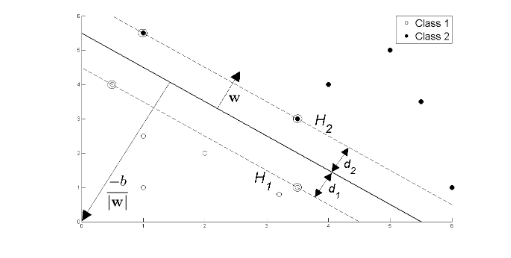
\includegraphics[scale = 0.7]{images/svm.png}
	    Figure: Hyperplane [4]
	\end{center}
	\begin{center}
	$w.x_i + b \geq +1$  for $y_i$=+1\\
	$w.x_i + b \leq -1 $ for $y_i$=-1    
	\end{center}
	We combine above two equations and we get;
	\begin{center}
	$y_i(w.x_i + b)-1 \geq 0$  for $y_i$=+1,-1\\
	\end{center}

	The two hyperplane H1 and H2 passing through the support vectors of +1 and -1 class respectively, so:
	\begin{center}
	w.x+b=-1 :H1\\
	w.x+b=1 :H2    
	\end{center}
	The distance between H1 hyperplane and origin is $\frac{(-1-b)}{|w|}$ and distance between H2 hyperplane and origin is $\frac{(1-b)}{|w|}$. So, margin can be given as
	\begin{center}
	M=$\frac{(1-b)}{|w|}$ - $\frac{(-1-b)}{|w|}$\\
	M=$\frac{2}{|w|}$
	\end{center}
	Where M is nothing but twice of the margin. So margin can be written as $\frac{1}{|w|}$. As, optimal hyperplane maximize the margin, then the SVM objective is boiled down to fact of maximizing the term $\frac{1}{|w|}$,
	Maximizing this term is equivalent to saying we are minimizing $|w|$ i.e. ( min($|w|$))
	or we can say min($\frac{||w||^2}{2}$) such that $y_i(w.x_i + b)-1 \geq 0$ for i =1...l

	SVM optimization problem is a case of constrained optimization problem, and it is always preferred to use dual optimization algorithm to solve such constrained optimization problem. That’s why we don’t use gradient descent.

	Lagrange method is required to convert constrained optimization problem into an unconstrained optimization problem. The goal of the above equation is to get the optimal value for w and b. So using Lagrange multipliers we can write the above expression as;
	\begin{center}
	    L = $\frac{||w||^2}{2} - \sum_{i=1}^{l} \lambda_i(y_i(w\cdot x_i+b)-1)$\\
	\end{center}
	\begin{equation}
	            L = \frac{||w||^2}{2} - \sum_{i=1}^{l} \lambda_i(y_i(w\cdot x_i+b))-\sum_{i=1}^{l}\lambda_i
	\end{equation}
	Now, we take the partial derivative of it with respect to w, b and $\lambda$.
	\begin{center}
	        $\frac{\partial l}{\partial w}$ = $w - \sum_{i=1}^{l} \lambda_i y_i x_i=0$\\
	        $\frac{\partial l}{\partial \lambda}$ = $ \sum_{i=1}^{l} y_i (w \cdot x_i+b)-1=0$\\
	        $\frac{\partial l}{\partial b}$ = $ \sum_{i=1}^{l} \lambda_i \cdot y_i=0$
	\end{center}
	From above we get:
	\begin{center}
	        w = $\sum_{i=1}^{l} \lambda_i y_i x_i$\\
	        $ \sum_{i=1}^{l} \lambda_i \cdot y_i=0$
	\end{center}

	From the above formulation we are able to find the optimal values of w only and it is dependent on $\lambda$, so we need to  also find the optimal value of $\lambda$. Finding the optimal value of b needs both w and $\lambda$. Hence, finding the value of $\lambda$ is important for us. Therefore, we do some algebraic manipulation:
	\\

	We substitute the value of w into equation 1. 

	\begin{center}
	$L_d = \frac{ (\sum_{i=1}^l\lambda_i \cdot y_i \cdot x_i)(\sum_{j=1}^l\lambda_j \cdot y_j \cdot x_j)}{2}-\sum_{j=1}^l\sum_{i=1}^l\lambda_j y_j(||\lambda_i \cdot y_i \cdot x_i||.x_j+b)+\sum_{i=1}^l \lambda_i$
	\end{center}
	\begin{center}
	    $L_d$ =$ \frac{(\sum_{i=1}^l\lambda_i \cdot y_i \cdot x_i)(\sum_{j=1}^l\lambda_j \cdot y_j \cdot x_j)}{2}-\sum_{j=1}^l\sum_{i=1}^l\lambda_j\lambda_i y_j y_i x_j x_i+\sum_{j=1}^l\sum_{i=1}^l\lambda_j y_j b+\sum_{i=1}^l \lambda_i$
	\end{center}
	Since our constraint was $\lambda_j \geq 0$ and $\sum_{j=1}^l\sum_{i=1}^l\lambda_j y_j$=0 so that term becomes zero. The first two terms get subtracted and after simplifying we have:
	\begin{center}
	    $L_d$ =$ \sum_{i=1}^l \lambda_i-\frac{1}{2}\sum_{j=1}^l\sum_{i=1}^l\lambda_j\lambda_i y_j y_i x_j x_i$
	\end{center}
	The optimization depends on the dot product of pairs of samples i.e. $x_i \cdot x_j$

	Now if the samples of our classes are not linearly separable then we transform our vectors to some other space and maximize the dot product of the transformation $\phi(x_j)\cdot\phi(x_i)$. Alternatively we use a function $K(x_i,x_j)=\phi(x_i)\cdot\phi(x_j)$ such that we don't need to know the transformation and this function gives us the dot product of the transformations in some space. This function in the context of SVMs is called a Kernel Function.
	\begin{center}
	    $L_d$ =$ \sum_{i=1}^l \lambda_i-\frac{1}{2}\sum_{j=1}^l\sum_{i=1}^l\lambda_j\lambda_i y_j y_i K(x_i, x_j)$
	\end{center}
	There are many kernel functions in SVM, so how to select a good kernel function is also a research issue. However, for general purposes, there are some popular kernel functions:\\

	1. Linear kernel: $K (x_i , x_j) = x_i^T\cdot x_j$ 

	2. Polynomial kernel: $K (x_i , x_j) = (\gamma x_i^T x_j + r)^d , \gamma > 0$ 

	3. RBF Kernel: $ K (x_i , x_j) = exp(-\gamma ||x_i - x_j||^2) , \gamma > 0$

	4.Sigmoid kernel:$ K (x_i , x_j) = tanh(\gamma x_i^T x_j + r)$  

	Here, $\gamma$, r and d are kernel parameters.[6]

\newpage
\section{Quantum Machine Learning Algorithms}
\subsection{Quantum Gradient Descent}
As seen in class, the Quantum Computing model was built up from the Classical model through a series of additions. In this section we will attempt to build up on the Classical model  of the Gradient Descent algorithm by first introducing the \textit{Stochastic Gradient Descent}, then moving on to discussing the various interpretations of a Quantum Gradient Descent that we observed during our research. 
\subsubsection{Stochastic Gradient Descent}
As we do in complexity theory it is important to consider the performance of our algorithm on a large value of N. This tells us how easy it is to scale the algorithm for bigger purposes. As data sets get larger, it becomes increasingly time consuming to perform Gradient Descent Algorithms on it as the algorithm iterates over the entire data set. Stochastic Gradient Descent makes use of random probabilistic approach of finding the minima of the function. Therefore, instead of performing the calculations over each point, a few samples are selected and the training model learns much quicker over larger data sets as argued by Wilson in \cite {BOOK:4}\cite {BOOK:5}

\subsection{Support Vector Machines via Grover's Algorithm}
During Research we encountered many versions of Quantum Support Vector Machines (QSVM) where each academic publication had its own approach with its own corresponding advantages and disadvantages. Implementing SVMs using quantum algorithms can result in exponential speedup over the classical implementations, potentially bringing the originally polynomial complexity down to a logarithmic complexity. 
\paragraph{}
\subsubsection{SVM's using Grover's Search Algorithm}
\textbf{Grover's Algorithm}
\paragraph{}
Grover's Algorithm is a searching algorithm that retrieves an element from an unordered quicker than it is possible using classical techniques. It offers a quadratic speed up on conventional search algorithms. Let us consider a blackbox function $f(x)$ where $f(x) = 0$ $\forall x$ such that $x\neq x_j$ and $f(x_j) = 1$. In order, for it to be invertible we must establish a function creates a one to one function for each bit string in the $2^N$ \textit(hilbert space). \paragraph{}
Suppose we have an $N bit$ string where $n = log(N)$. We apply a Hadamard Transform on $|0\rangle^{\odot n}$ to obtain an equal superimposed state: 
$$|\psi\rangle = \frac{1}{\sqrt{n}}\sum_{n=0}^{n-1}|x\rangle$$

\subsubsection{Exponential Speedup of SVM through Quantum Means}

\begin{enumerate}
	\item Quantum Matrix Inversion
\end{enumerate}
\newpage
\section{Quantum Neural Networks}
\newpage

% \section{Reflection}
% \subsection{Advantages of Quantum Machine Learning}
% \subsection{Current Limitations}
% \subsection{Future Prospects}
% \newpage
% \section{Bibliography}
% \begin{enumerate}
%     \item \url{https://kkpatel7.files.wordpress.com/2015/04/alppaydin_machinelearning_2010.pdf}
%     \item \url{https://www.researchgate.net/publication/225151243_Machine_Learning_in_a_Quantum_World}
    
%     \item \url{https://medium.com/@ankitnitjsr13/math-behind-support-vector-machine-svm-5e7376d0ee4d}
%     \item \url{https://towardsdatascience.com/support-vector-machine-introduction-to-machine-learning-algorithms-934a444fca47}
%     \item \url{http://www.jatit.org/volumes/research-papers/Vol12No1/1Vol12No1.pdf?fbclid=IwAR0xhouaOTffxsjwMCONzZeOubmQWl3PfZH94AUXMCNbfpBWKQaDbSBefNI}
%     \item \url{https://arxiv.org/pdf/1909.05074.pdf}
%     \item \url{https://arxiv.org/pdf/1909.02108.pdf}  
%     \item \url{https://arxiv.org/pdf/0905.2794.pdf}
%     \item \url{https://iopscience.iop.org/article/10.1088/1367-2630/ab2a9e/pdf}
    
% \end{enumerate}


\bibliography{Report}
\bibliographystyle{ieeetr}
\section{Glossary}


\end{document}